\documentclass[tikz,border=3mm]{standalone}

\usepackage{pgfplots}
\usetikzlibrary{shapes.misc, positioning}

\usetikzlibrary{decorations.pathreplacing}
\usetikzlibrary{calc}
\usetikzlibrary{chains}
\usetikzlibrary{shapes}


\usepackage{xcolor}

\definecolor{g1}{RGB}{90, 200, 94}
\definecolor{g2}{RGB}{113, 200, 55}
\definecolor{g3}{RGB}{170, 222, 135}
\definecolor{g4}{RGB}{200, 250, 175}
\definecolor{strange}{RGB}{210,224,233}


\makeatletter
\def\grd@save@target#1{%
  \def\grd@target{#1}}
\def\grd@save@start#1{%
  \def\grd@start{#1}}
\tikzset{
  grid with coordinates/.style={
    to path={%
      \pgfextra{%
        \edef\grd@@target{(\tikztotarget)}%
        \tikz@scan@one@point\grd@save@target\grd@@target\relax
        \edef\grd@@start{(\tikztostart)}%
        \tikz@scan@one@point\grd@save@start\grd@@start\relax
        \draw[minor help lines] (\tikztostart) grid (\tikztotarget);
        \draw[major help lines] (\tikztostart) grid (\tikztotarget);
        \grd@start
        \pgfmathsetmacro{\grd@xa}{\the\pgf@x/1cm}
        \pgfmathsetmacro{\grd@ya}{\the\pgf@y/1cm}
        \grd@target
        \pgfmathsetmacro{\grd@xb}{\the\pgf@x/1cm}
        \pgfmathsetmacro{\grd@yb}{\the\pgf@y/1cm}
        \pgfmathsetmacro{\grd@xc}{\grd@xa + \pgfkeysvalueof{/tikz/grid with coordinates/major step}}
        \pgfmathsetmacro{\grd@yc}{\grd@ya + \pgfkeysvalueof{/tikz/grid with coordinates/major step}}
        \foreach \x in {\grd@xa,\grd@xc,...,\grd@xb}
        \node[anchor=north] at (\x,\grd@ya) {\pgfmathprintnumber{\x}};
        \foreach \y in {\grd@ya,\grd@yc,...,\grd@yb}
        \node[anchor=east] at (\grd@xa,\y) {\pgfmathprintnumber{\y}};
      }
    }
  },
  minor help lines/.style={
    help lines,
    step=\pgfkeysvalueof{/tikz/grid with coordinates/minor step}
  },
  major help lines/.style={
    help lines,
    line width=\pgfkeysvalueof{/tikz/grid with coordinates/major line width},
    step=\pgfkeysvalueof{/tikz/grid with coordinates/major step}
  },
  grid with coordinates/.cd,
  minor step/.initial=.2,
  major step/.initial=1,
  major line width/.initial=2pt,
}

\makeatother

\usepackage{etoolbox}
\newcounter{mylistcounter}

\def\saveitem#1{%
\stepcounter{mylistcounter}%
\expandafter\def\csname mylist\themylistcounter\endcsname{#1}}

\forcsvlist{\saveitem}{%
   1,
   i,
   nsp
}%


\def\getnthelement#1{\csname mylist#1\endcsname}


\usepackage{ifthen}


\begin{document}

\tikzset{
        kernel/.pic={
        \foreach \i in {5,4.5,...,0.5}{
            {\fill[gray!50] (\i, 5-\i) -- (5,5-\i) -- (5,5) -- (\i,5);}
        }
        \draw (0,0) grid[step=.5] (5,5);
    }
}

\tikzset{
    kernf/.pic={
        \fill[white] (0, 0) -- (5,0) -- (5,5) -- (0,5) -- cycle;
    }
}


\begin{tikzpicture}

    \draw[opacity = 0.1](3,-3) pic {kernel};
    \draw[opacity = 0.2](2,-2) pic {kernel};
    \draw[opacity = 0.3](1,-1) pic {kernel};

    \begin{scope}
                \foreach \i in {3,2.5,...,0}{
                    {\fill[blue!50] (\i, 5-\i-2) -- (5,5-\i-2) -- (5,5) -- (\i,5);}
            }
        \foreach \i in {4,3.5,...,0}{
                    {\fill[red!50] (\i, 5-\i-1) -- (5,5-\i-1) -- (5,5) -- (\i,5);}
            }
        \foreach \i in {5,4.5,...,0.5}{
                    {\fill[gray!50] (\i, 5-\i) -- (5,5-\i) -- (5,5) -- (\i,5);}
            }
        
        \draw (0,0) grid[step=.5] (5,5);
        \draw (2.5,5) node[above]{$size_t$} ;
        \draw (0,2.5) node[left]{$size_{t+1}$} ;
        \draw(0,5) node[above] {$L$};
        \draw(5,5) node[above] {$U$};
        
        \draw(7,5) node[fill=red!50,above] {Gauss-Legendre};
        \draw(7,5) node[fill=blue!50,below] {Midbin};
        \draw[->] (0, -0.5) -- (2.5,-3);
        \draw(1,-1.5) node[below, rotate = -45] {Basal Area};
    \end{scope}

\end{tikzpicture}

\def\r{0.2}

\begin{tikzpicture}

    % \draw (-7,-17) to[grid with coordinates] (15, 1);

    \node at (0,0) (forest) {};
    \draw [rounded corners, fill = g1!60] (forest) rectangle +(14.2, -16.6) {};
    \node [below right=\r cm and \r cm of forest] { \textbf{Forest class} (community/plot)};

    \node at (\r, -1.2) (harvr) {};    \node at (2*\r + 9, -1.2) (infoF) {}; 
    \draw [rounded corners, dashed] (harvr) rectangle node[text width=12cm, align= center]{
        \textbf{harv\_rules} $[$\scriptsize Pmax, dBAmin, freq, alpha\normalsize $]$ } +(9, -1);
        
    \draw [rounded corners, dotted] (infoF) rectangle node[text width = 4.6cm, align= center]{
        \textbf{info} list \\ \scriptsize Species name and clim\_lab \normalsize } +(4.6, -1);

    \begin{scope}[xshift = 2*\r cm, yshift = -2.8 cm]

    \node at (-\r, \r) (species) {};
    \draw [rounded corners, dotted] (species)rectangle +(13.8, -13.8) {};

    \node at (0, 0) (speciesB) {};
    % \draw [rounded corners] (speciesB)rectangle +(13.4, -13.2) {};
    \draw [rounded corners, fill = g2!60] (speciesB) -- (4,0) -- (4,-1) -- (13.4,-1) -- (13.4, -13.4) -- (0, -13.4)  -- cycle;
    \node [below right=\r cm and \r cm of speciesB] {\textbf{Species class}};

    \node at (4.2, 0) (sp1) {};           \node at (4.2 + 3.2, 0) (sp2) {}; 

    \draw [rounded corners, fill = g2!60] (sp1) rectangle node{Species A} +(3, -0.8);
    \draw [rounded corners, fill = g2!60] (sp2) rectangle node{Species B} +(3, -0.8);

    % layout
    \begin{scope}[xshift = \r cm, yshift = -1.2 cm]
    \node at (0, 0) (init) {};    \node at (4.2 + \r , 0) (recruit) {};
    \node at (0, -\r -1) (harv) {};   \node at (4.2 + \r , -\r - 1) (harvl) {};  \node at (3.4 + 4.2 + 2*\r , -\r - 1) (rdi) {};
    \node at (0, -2*\r -2) (dist) {};   \node at (5.6 + \r , -2*\r - 2) (distc) {};
    

    \draw [rounded corners, loosely dashdotted] (init) rectangle node[text width=4.2cm, align= center]{
        \textbf{init\_pop}(\scriptsize mesh, SurfEch\normalsize) } +(4.2, -1);
    \draw [rounded corners, loosely dashdotted] (recruit) rectangle node[text width=8.6cm, align= center]{
        \textbf{recruit\_fun}(\scriptsize BATOTSP, BATOTNonSP, mesh, SurfEch\normalsize) } +(8.6, -1);

    \draw [rounded corners, loosely dashdotted] (harv) rectangle node[text width=4.2cm, align= center]{
        \textbf{harv\_fun}(\scriptsize x, species, ...\normalsize) } +(4.2, -1);
    \draw [rounded corners, dashed] (harvl) rectangle node[text width=3.4cm, align= center]{
        \textbf{harv\_lim} vector } +(3.4, -1);
    \draw [rounded corners, dashed] (rdi) rectangle node[text width=3.4cm, align= center]{
        \textbf{rdi\_coef} vector } +(3.4, -1);

    \draw [rounded corners, loosely dashdotted] (dist) rectangle node[text width=5.6cm, align= center]{
            \textbf{disturb\_fun}(\scriptsize x, species, disturb, ...\normalsize) } +(5.6, -1);
    \draw [rounded corners, dashed] (distc) rectangle node[text width=5.6cm, align= center]{
        \textbf{disturb\_coef} vector } +(5.6, -1);
    
    \end{scope}

    

    \begin{scope}[xshift = \r cm, yshift = -5 cm] % IPM class
    \node at (0, 0) (IPM) {};
    \draw [rounded corners, fill = g3!60] (IPM) rectangle +(13, -8.2) {};
    \node [below right=\r cm and \r cm of IPM] {\textbf{IPM class}, matrices after integration from fitted models};

    \begin{scope}[xshift = \r cm, yshift = -1 cm]

        \begin{scope}
            % IPM matrices scope
            \node at (0, 0) (IPM) {};
            \draw [rounded corners, dotted] (IPM) rectangle +(6, -3.4);
            \node [below right=\r cm and \r cm of IPM] (mlab) {\textbf{Growth * Mortality} matrices};
    
            % layout
            \node [below left=1.5 cm and 0cm of mlab] (k1) {};
            \node [below right= \r/2 cm and \r cm of k1] (k2) {};
            \node [below right= \r/2 cm and \r cm of k2] (k3) {};

            \draw pic[scale = 0.3] at(k3) {kernf};
            \draw pic[scale = 0.3, opacity = 0.2] at(k3) {kernel};
            \draw pic[scale = 0.3] at(k2) {kernf};
            \draw pic[scale = 0.3, opacity = 0.3] at(k2) {kernel};
            \draw pic[scale = 0.3] at(k1) {kernf};
            \draw pic[scale = 0.3, opacity = 0.6] at(k1) {kernel};
            \node [above right= -3*\r cm and 2.5 cm of k1, text width=3cm,align=center] {
            Dimensions: \\ $m * m * BA$ \\~\\ Names : $BA$ \tiny\\$m = length(mesh)$};
        \end{scope}


        \begin{scope}[xshift = 6.2 cm]
            % scope for simple vectors
            % layout
            \node at (0, 0) (BAv) {};           \node at (3.2, 0) (mv) {};
            \node at (0, -\r - 1) (cliv) {};    
            \node at (0, -2*\r - 2) (intv) {};  

            \draw [rounded corners, dashed] (BAv) rectangle node{\textbf{BA} vector} +(3, -1);
            \draw [rounded corners, dashed] (mv) rectangle node{\textbf{mesh} vector} +(3, -1);
            \draw [rounded corners, dashed] (cliv) rectangle node{\textbf{climatic} vector : named clim variable} +(6.2, -1);
            \draw [rounded corners, dashed] (intv) rectangle node{\textbf{int} vector : log of integration param} +(6.2, -1);

        \end{scope}
    
        \begin{scope}[xshift = 0 cm, yshift = -3.6 cm]
            \node at (0,0) (fit) {};
            \draw [rounded corners, fill = g4!60] (fit) rectangle +(8.6, -3.4);
            \node [below right=\r cm and \r cm of fit] {
                \textbf{Fit class} (function params)
            };
            \node at (\r, -1.2) (sv) {};
            \draw [rounded corners, dotted] (sv)rectangle node{\textbf{Survival}} +(2.5, -1);
            \node [right= 2.5 cm of sv] (gr) {};
            \draw [rounded corners, dotted] (gr) rectangle node{\textbf{Growth}} +(2.2, -1);
            \node [right= 2.2 cm of gr] (rec) {};
            \draw [rounded corners, dotted] (rec) rectangle node{\textbf{Recruitment}} +(3, -1) ;
        
            \node [below right= 1.2 cm and \r cm of sv] {species name and $max\_dbh$};
    
        \end{scope}

        \node at (8.6 + \r, -3*\r - 3) (infv) {};
        \draw [rounded corners, dashed] (infv) rectangle node[text width=3cm, align= center]{
            \textbf{info} vector \\~\\ species name, \\ correction, clim\_lab, surv, compress, delay} +(3.6, -3.4);
    
    \end{scope}

\end{scope}

\end{scope}

\begin{scope}[xshift = -6.6 cm, yshift = -1cm]
    % Légende
    % layout
    \node at (0, 0) (class) {};           \node at (3.2, 0) (list) {};
    \node at (0, -\r - 1) (vector) {};    \node at (3.2, -\r - 1) (fun) {};

    \node[above right= 0cm and 0cm of class] {\textbf{Legend}};
    \draw [rounded corners] (class) rectangle node{\textbf{S3 Class} object} +(3, -1);
    \draw [rounded corners, dashed] (vector) rectangle node{\textbf{vector} object} +(3, -1);
    \draw [rounded corners, dotted] (list) rectangle node{\textbf{list} object} +(3, -1);
    \draw [rounded corners, loosely dashdotted] (fun) rectangle node{\textbf{function()}} +(3, -1);

\end{scope}


\end{tikzpicture}


\tikzset{
    recp/.pic={
        \draw (0.2, 1) node[circle,minimum size=2cm] (p) {};
        \draw (-0.2,-0.1) node[fill = strange,circle,minimum size=0.5cm] (p1) {};
        \draw node[above right = 0.5cm and 0.1 cm of p1,
         fill = strange,circle,minimum size=0.5cm] (p2) {};
        \draw node[above right = -0.2cm and 0.5 cm of p1,
        fill = strange,circle,minimum size=0.5cm] (p3) {};
    }
}

\def\nsp{3}

\begin{tikzpicture}[
    block/.style={draw,fill=strange,minimum height=2.5em},
    ncirc/.style={fill = strange,circle,minimum size=2cm},
    font=\sffamily,>=stealth]

    % Single species functions
    \begin{scope}[start chain=A going below,node distance=3cm,
    local bounding box=buffers]
    \foreach \X in {1,...,\nsp}
    {

    \ifthenelse{\equal{\X}{1}}{\def\sop{1}}{\def\sop{0.3}}

    \draw node[ncirc, on chain] (nzt-\X) {$n(s_{\getnthelement{\X}},z,t)$};

    \draw node[right= 4cm of nzt-\X, ncirc, opacity = \sop] (ng-\X) {};
    \draw node[right= 3cm of ng-\X, ncirc, opacity = \sop] (nh-\X) {};
    \draw node[right= 3cm of nh-\X, ncirc, opacity = \sop] (nd-\X) {};
    \draw node[right= 3cm of nd-\X, ncirc, draw] (nr-\X) {$n(s_{\getnthelement{\X}},z,t+1)$};

    \draw[->, thick, opacity = \sop](nzt-\X) edge node[midway, above](ngf-\X){Growth $\times$ Mortality} (ng-\X);
    \draw[->, thick, opacity = \sop](ng-\X) edge node[midway, above](nhf-\X){Harvesting} (nh-\X);
    \draw[->, thick, opacity = \sop](nh-\X) edge node[midway, above]{Disturbance} (nd-\X);
    \draw[->, thick, opacity = \sop](nd-\X) edge node[midway, above](rec-\X){Recruitment} (nr-\X);

    \node[below right= 1.5cm and 0.1 cm of rec-\X] (recp-\X) {};
    \draw pic[below= 2.2cm of rec-\X, opacity = \sop] {recp};
    \draw[->, thick, opacity = \sop](p) edge node[midway]{} (nr-\X);
    \draw[->, thick, opacity = \sop](nd-\X) edge node[midway]{} (p);

    \draw node[below= 0.5cm of nh-\X, ncirc, draw] (harv-\X) {$h(s_{\getnthelement{\X}},z,t)$};
    \draw[->, thick, opacity = \sop](nhf-\X) edge node[midway]{} (harv-\X);

    }
    \end{scope} 

    % Common node with BA computation
    \node[right=2cm of buffers,align=center,inner sep=0.5pt,fill=strange,
        circle] (cBA) {$\sum_{i=1}^{nsp} n(s_i, z, t+1)$};
    \draw node[right= 3cm of cBA, ncirc, draw] (BA) {BATOTSP};
    \draw[->, thick](cBA) edge node[midway, fill=white]{Compute BA} (BA);
    % arros from nt+1 to BA
    \foreach \X in {1,...,\nsp} 
    {
        \draw[->,thick] (nr-\X.east) --  ++ (1cm,0) -- (cBA);
    }

    % get sim ipm
    \begin{scope}[start chain=A going below,node distance=3cm,
        local bounding box=buffers]
        \foreach \X in {1,...,\nsp}
        {

        \ifthenelse{\equal{\X}{1}}{\def\sop{1}}{\def\sop{0.3}}
        \draw node[right= 13cm of nr-\X, ncirc, fill = white] (getipm-\X) {};
        \draw pic[below left= 0cm and 0cm of getipm-\X, scale = 0.3, opacity = \sop]  {kernel};
        \draw[<-,thick, opacity = \sop] (getipm-\X.west) -- node[above](s){$get\_sim\_ipm()$} ++(-2.5cm, 0) -- (BA);
        }
    \end{scope} 

    % print ipm list
    \begin{scope}[shift={($(getipm-1.west)+(-5.2cm,-0.5cm)$)}]
        \node at (1, 1.8) {$s_i$ IPMs};
        \draw (0.8,-0.4) pic[scale = 0.3, opacity = 0.2]  {kernel};
        \draw (0.4,-0.2) pic[scale = 0.3] {kernf};
        \draw (0.4,-0.2) pic[opacity = 0.4, scale = 0.3]  {kernel};
        \draw (0,0) pic[scale = 0.3] {kernf};
        \draw (0,0) pic[opacity = 0.6, scale = 0.3]  {kernel};
    \end{scope} 

    % BATOTNON sp arrows
    \draw node[right= 4cm of nr-1, ncirc] (bansp-1) {\scriptsize BATOTNONSP};
    \draw[->,thick] (nr-1) -- (bansp-1);
    \draw[->,thick] (BA) -- (bansp-1);
    \draw[->,thick, loosely dotted] (bansp-1.north) -- ++ (0,1cm) -- ($(rec-1.north)+(0,1.5cm)$) -- (rec-1.north);

    % retroaction arrow of the IPM
    \draw[->,thick, loosely dotted] (getipm-1.north) -- ++ (0,1.5cm) -- ($(ngf-1.north)+(0,2.1cm)$) -- (ngf-1.north);


    \begin{scope}[xshift = -8 cm, yshift = -1cm]
        % Légende
        % layout
        \node at (0, 0) (size) {};          
        \node at (2.3, 0) (out) {}; 
        
        \node at (-1, -2.5) (as) {};  \node at (4, -2.5) (ae) {};
        \node at (-1, -3.5) (ds) {};  \node at (4, -3.5) (de) {}; 
    
        \node[above right= 1cm and -1cm of size] {\textbf{Legend}};
        \draw node[ncirc] at (size) { \scriptsize Size distribution};
        \draw node[ncirc, draw] at (out) { \scriptsize Saved output};
        \draw[->, thick](as) edge node[midway, above, fill=white]{Function} (ae);
        \draw[->, thick, dotted](ds) edge node[midway, fill=white]{Retroaction at $t+1$} (de);
    
    \end{scope}
    

\end{tikzpicture}

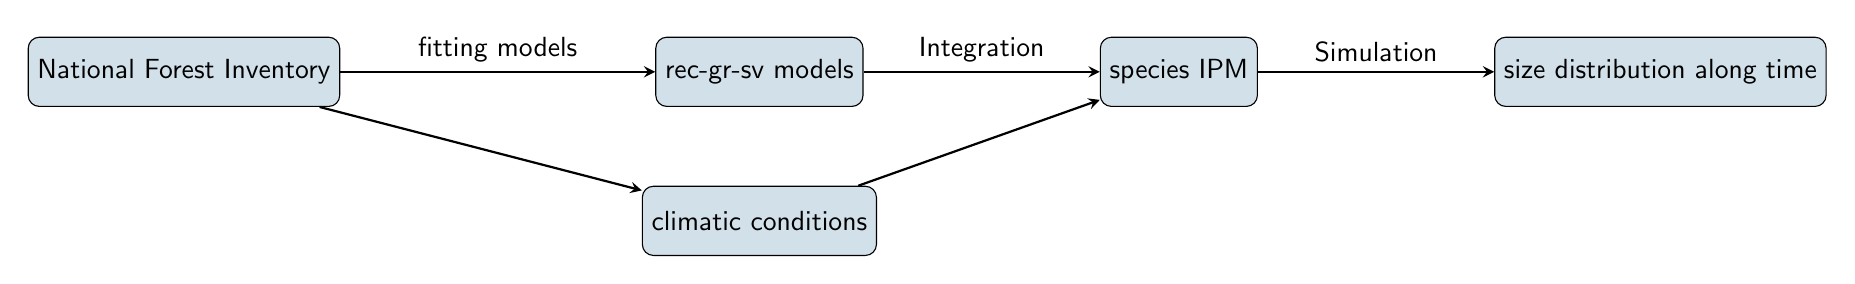
\begin{tikzpicture}[
    block/.style={draw,fill=strange,minimum height=2.5em, rounded corners},
    font=\sffamily,>=stealth]
    \draw node[block] (nfi) {National Forest Inventory};

    \draw node[right= 4cm of nfi, block] (mod) {rec-gr-sv models};
    \draw node[below= of mod, block] (cli) {climatic conditions};
    \draw node[right= 3cm of mod, block] (ipm) {species IPM};
    \draw node[right= 3cm of ipm, block] (sim) {size distribution along time};

    \draw[->, thick](nfi) edge node[midway, above](ngf){fitting models} (mod);
    \draw[->, thick](nfi) edge (cli);
    \draw[->, thick](cli) edge (ipm);
    \draw[->, thick](mod) edge node[midway, above](nhf){Integration} (ipm);
    \draw[->, thick](ipm) edge node[midway, above]{Simulation} (sim);
\end{tikzpicture}

\end{document}